\selectlanguage{english}
\chapter{Project Context and State of the Art}
\renewcommand{\chaptername}{Chapter}

\section*{Introduction}
\addcontentsline{toc}{section}{\textbf{Introduction}}

This chapter situates the project within the transformation of information access
driven by generative AI. It traces the shift from traditional search to answer-based
generation, motivates the growing importance of LLM visibility for local businesses,
and formulates the core problem. It then defines the project objectives, reviews the
relevant state of the art, and identifies the gaps the proposed system addresses.

% ─────────────────────────────────────────────
\section{Context and Motivation}

The way users access information has undergone a fundamental transformation. The
rapid adoption of conversational AI systems — ChatGPT, Gemini, Perplexity — has
shifted the dominant paradigm from \textit{link-based retrieval}, where users select
from a ranked list of sources, to \textit{answer-based generation}, where the system
synthesizes a direct response. A user asking \textit{``Where should I eat tonight in
Tunis?''} may now receive a curated set of recommendations presented as authoritative
text, without consulting any external source.

This shift has direct commercial consequences. Visibility in an AI-generated response
has become as commercially relevant as a first-page search ranking. Unlike traditional
SEO signals — backlinks, keywords, structured markup — which are documented and
actionable, LLM outputs are generated by probabilistic models whose entity selection
mechanisms are not directly observable. A business consistently mentioned benefits
from significant exposure; one never mentioned effectively does not exist within this
emerging information channel.

This situation motivates a new discipline: \textbf{Generative Engine Optimization
(GEO)}, defined as the study of how entities are represented, measured, and
potentially optimized within LLM-generated responses~\cite{aggarwal2023geo}. GEO is
particularly relevant for local businesses in markets such as Tunisia, where limited
digital footprints and low representation in web corpora create a structural
disadvantage in model training data.

% ─────────────────────────────────────────────
\section{Problem Statement}

\subsection*{The Visibility Crisis in the Age of Generative AI}

The widespread adoption of LLMs as everyday information tools is reshaping how
businesses are discovered. ChatGPT surpassed 100 million active users within two
months of launch~\cite{aggarwal2023geo} — an adoption pace unprecedented in consumer
technology. As conversational AI becomes the primary interface for local discovery,
a commercial reality emerges: \textit{if a business does not appear in an LLM's
response, it does not exist for that user}.

Unlike a search engine, which indexes content in near real-time, an LLM encodes
knowledge statically during pre-training. Entities that were prominent and richly
documented in the training corpus are reliably recalled; entities that were absent or
sparse are structurally neglected, regardless of their actual quality. As LLM usage
scales, this asymmetry compounds: every confident recommendation for one brand
implicitly excludes equally deserving competitors the model has no knowledge of.

The consequences are disproportionately severe for local businesses. Large
international chains benefit from accumulated web presence — review aggregators, news
coverage, Wikipedia articles, social media mentions — all contributing to robust
training data representation. A small Tunisian restaurant with no Wikipedia page,
minimal reviews, and limited social reach remains invisible to the model, and by
extension, to the growing share of users who discover businesses through AI-generated
recommendations. Brands that start invisible risk remaining so, locked out of a
feedback loop they cannot enter without first being visible.

\subsection*{The Measurement and Optimization Gap}

Compounding this structural problem is the absence of any reliable methodology to
measure or act upon LLM-based visibility. The stochastic nature of LLM inference
means that a business may appear in 60\% of responses to a given query and be absent
from the remaining 40\%. Without repeated, systematic measurement, this variability
is invisible. A single query gives no actionable signal.

As a result, a business owner in this environment faces three compounding deficits:

\begin{itemize}[label=\textbullet]
    \item \textbf{No visibility audit:} no tool reliably determines how often, in
    what contexts, and with what accuracy an LLM mentions their business.

    \item \textbf{No benchmarking:} without cross-entity comparison, a business
    cannot assess its relative position within its competitive landscape as perceived
    by generative models.

    \item \textbf{No optimization pathway:} without understanding which web presence
    signals correlate with LLM visibility, a business cannot take informed action.
\end{itemize}

This triple deficit limits both practical decision-making and the scientific
understanding of how entity representation in generative systems relates to
observable web presence. Addressing it requires autonomous multi-source data
collection, statistically rigorous cross-model measurement, and structured analytical
output — the precise problem this project is designed to solve.

% ─────────────────────────────────────────────
\section{Project Objectives and Scope}

This project aims to design and implement an autonomous multi-agent pipeline for
measuring brand visibility in LLM-generated responses. Three objectives guide its
development:

\begin{itemize}[label=\textbullet]
    \item \textbf{O1.} Measure the consistency with which named entities appear in
    LLM-generated responses across varied prompts and models.

    \item \textbf{O2.} Acquire and structure multi-source web presence data
    associated with identified entities.

    \item \textbf{O3.} Construct an analytical dataset enabling the study of
    relationships between LLM visibility signals and web presence features.
\end{itemize}

Two research questions guide the investigation:

\begin{itemize}[label=\textbullet]
    \item \textbf{RQ1.} How consistently do LLMs mention local businesses across
    repeated queries?

    \item \textbf{RQ2.} What web presence features are associated with higher
    visibility in LLM-generated responses?
\end{itemize}

The pipeline is applied to the Tunisian restaurant sector using French-language
prompts. Real-time monitoring and GEO optimization recommendations fall outside
the scope of this project.

% ─────────────────────────────────────────────
\section{Literature Review and State of the Art}

\subsection{Search Engine Optimization}

Since the late 1990s, Search Engine Optimization has been the dominant framework for
managing online visibility. The foundational mechanism is the PageRank algorithm
introduced by Brin and Page in 1998~\cite{brin1998anatomy}, which ranks pages by the
number and quality of inbound links. Over the following decades, SEO evolved to
encompass technical optimization (site speed, crawlability, structured markup),
on-page content quality, and off-page authority signals~\cite{moz2023seo}.

However, SEO operates under a fundamental assumption: the user receives a ranked list
of links and selects one. This assumption no longer holds when the system generates a
synthesized answer directly. The signals that drove traditional SEO become insufficient
as measures of visibility in AI-generated responses — the central challenge addressed
by this project.

% ─────────────────────────────────────────────
\subsection{Generative AI in Information Retrieval and the Emergence of GEO}

The introduction of the Transformer architecture~\cite{vaswani2017attention} and the
public release of capable models — ChatGPT, Gemini, LLaMA~\cite{touvron2023llama},
Mistral~\cite{jiang2023mistral} — established a rapidly evolving landscape of
generative systems available through commercial APIs and open-source releases.

The concept of \textbf{Generative Engine Optimization (GEO)}, formally introduced by
Aggarwal et al.\ in 2023~\cite{aggarwal2023geo}, addresses what determines whether a
given entity appears in an LLM-generated response. GEO differs from SEO in a
fundamental way: SEO operates on a crawlable, indexed web with observable ranking
signals. GEO targets systems that encode knowledge implicitly during pre-training,
with no index to rank in and no direct feedback signal. Visibility is an emergent
property of how well an entity is represented across the web sources that formed the
model's training data. Table~\ref{tab:seo_vs_geo} summarizes the key distinctions.

\begin{table}[H]
\centering
\renewcommand{\arraystretch}{1.6}
\setlength{\tabcolsep}{8pt}
\begin{tabularx}{\textwidth}{
    >{\raggedright\bfseries\arraybackslash}p{2.8cm}
    >{\centering\arraybackslash}X
    >{\centering\arraybackslash}X
}
\rowcolor{white}
&
\cellcolor{seopurple}\textcolor{white}{\textbf{SEO\newline(Search Engine Optimisation)}} &
\cellcolor{geoblue}\textcolor{white}{\textbf{GEO\newline(Generative Engine Optimisation)}} \\
\midrule
\rowcolor{rowgray}
Target Platforms &
\cellcolor{seolightpurple} Traditional search engines: Google, Bing, Yahoo. &
\cellcolor{geolightblue} AI-driven engines: ChatGPT, Gemini, Perplexity, DeepSeek. \\
\rowcolor{white}
Ranking Method &
\cellcolor{seolightpurple} Algorithm-based ranking: keywords, links, technical performance. &
\cellcolor{geolightblue} AI synthesis based on training data representation and content quality. \\
\rowcolor{rowgray}
Key Metrics &
\cellcolor{seolightpurple} Organic traffic, keyword rankings, CTR, backlink profile. &
\cellcolor{geolightblue} Inclusion rate in AI responses, citation frequency. \\
\rowcolor{white}
User Behaviour &
\cellcolor{seolightpurple} Users click through to the website for answers. &
\cellcolor{geolightblue} Users consume information directly within the AI's response. \\
\rowcolor{rowgray}
Update Frequency &
\cellcolor{seolightpurple} Influenced by search engine algorithm updates. &
\cellcolor{geolightblue} Influenced by AI model training cycles. \\
\bottomrule
\end{tabularx}
\caption{Comparison of SEO and GEO across key dimensions. Adapted from~\cite{aggarwal2023geo}.}
\label{tab:seo_vs_geo}
\end{table}

Early empirical work on GEO identified content-level signals associated with higher
mention rates: authoritative citations, fluent prose, and domain-specific
terminology~\cite{aggarwal2023geo}. However, this work focused on document-level
optimization, leaving unanswered how \textit{entity-level} web presence — structured
data on review platforms, social media, and knowledge bases — correlates with
visibility in generative responses.

% ─────────────────────────────────────────────
\subsection{Large Language Models and Entity Representation}

LLMs acquire knowledge about entities implicitly during pre-training on large text
corpora. Unlike a database, an LLM does not store facts explicitly; it encodes
statistical associations across billions of training examples. The frequency and
consistency with which an entity appears in training data directly influences how
reliably the model recalls and mentions it~\cite{mallen2023trust}.

This \textbf{frequency bias} has been empirically demonstrated by Mallen et al.\
(2023): LLMs are significantly more accurate when recalling popular, frequently
referenced entities than rare or locally known ones~\cite{mallen2023trust}. Beyond
frequency, two additional risks apply: \textbf{hallucination} — the generation of
plausible but factually incorrect entity information~\cite{ji2023hallucination} —
and \textbf{representation inconsistency}, where the same entity is described
differently across runs of the same prompt. Both are pronounced for entities with
sparse training data coverage, making systematic multi-run measurement essential.

% ─────────────────────────────────────────────
\subsection{Agentic AI Systems and Multi-Agent Architectures}

An AI agent is a system that perceives its environment, reasons about its current
state, selects actions, and executes them in pursuit of a goal~\cite{russell2020ai}.
LLMs capable of multi-step reasoning and external tool use have enabled agents that
autonomously decompose complex goals into executable steps.

\paragraph{The ReAct Framework.}
The \textbf{ReAct} framework~\cite{yao2022react} grounds LLM reasoning in external
reality by interleaving reasoning traces with action steps — calls to external tools
or APIs. At each step the agent produces a \textit{thought}, selects an
\textit{action} (a tool call with structured arguments), and receives an
\textit{observation} (the tool's response). This cycle repeats until sufficient
information has been gathered. Figure~\ref{fig:react_loop} illustrates the loop.

\begin{figure}[ht]
\centering
\begin{tikzpicture}[
  node distance=1.2 cm and 2.4 cm,
  thought/.style={rectangle, rounded corners=4pt, draw=blue!60, fill=blue!8,
                  text width=3cm, align=center, font=\small, minimum height=0.8cm},
  action/.style={rectangle, rounded corners=4pt, draw=orange!70, fill=orange!8,
                 text width=3cm, align=center, font=\small, minimum height=0.8cm},
  obs/.style={rectangle, rounded corners=4pt, draw=teal!60, fill=teal!7,
              text width=3cm, align=center, font=\small, minimum height=0.8cm},
  env/.style={rectangle, rounded corners=4pt, draw=gray!60, fill=gray!8,
              text width=2.8cm, align=center, font=\small, minimum height=1.4cm,
              dashed},
  io/.style={rectangle, rounded corners=4pt, draw=green!60!black, fill=green!7,
             text width=2.8cm, align=center, font=\small, minimum height=0.8cm},
  arrow/.style={-{Stealth[length=5pt]}, thick},
]
\node[io] (task) {Task / Question};
\node[thought, below=0.9cm of task]    (thought) {\textbf{Thought}\\Reasoning step};
\node[action,  below=1.1cm of thought] (action)  {\textbf{Action}\\Tool invocation};
\node[obs,     below=1.1cm of action]  (obs)     {\textbf{Observation}\\Tool result};
\node[io, below=0.9cm of obs] (answer) {Answer / Output};
\node[env, right=2.6cm of action] (env)
  {\textbf{External}\\\textbf{Environment}\\[4pt]
   \footnotesize Search, KG,\\Calculator, API\ldots};
\draw[arrow] (task)    -- (thought);
\draw[arrow] (thought) -- (action);
\draw[arrow] (action)  -- (obs);
\draw[arrow] (obs)     -- (answer);
\draw[arrow, bend left=50]
  (obs.west) to node[left, font=\scriptsize, text width=1.2cm, align=center]
  {next\\reasoning\\step} (thought.west);
\draw[arrow] (action.east) -- node[above, font=\scriptsize] {query}  (env.west);
\draw[arrow] (env.south)   -- node[right, font=\scriptsize] {result}
  (env.south |- obs.east) -- (obs.east);
\node[font=\scriptsize, text=gray, right=0.1cm of answer] {(when done)};
\node[font=\scriptsize, text=gray, right=0.1cm of task]   {(initial input)};
\node[draw=blue!30, dashed, rounded corners=6pt,
      fit=(thought)(action)(obs), inner sep=8pt,
      label={[font=\footnotesize\itshape, blue!60]above:ReAct Loop}] {};
\end{tikzpicture}
\vspace{0.5cm}
\caption{The ReAct framework~\cite{yao2022react}: the agent alternates between
\textit{Thought}, \textit{Action}, and \textit{Observation}, iterating until a
final answer is produced.}
\label{fig:react_loop}
\end{figure}

\paragraph{Multi-Agent Orchestration.}
Complex pipelines benefit from distributing responsibility across multiple specialized
agents coordinated by an orchestrating layer. As shown in
Figure~\ref{fig:agent_evolution}, the field has progressed from single agents to
fully orchestrated systems with a dedicated coordination layer. The key distinction
is between \textbf{fixed pipelines} — executing a predetermined sequence regardless
of intermediate results — and \textbf{autonomous orchestrators} — which reason about
the current state at each step and determine the next action dynamically.

\begin{figure}[H]
    \centering
    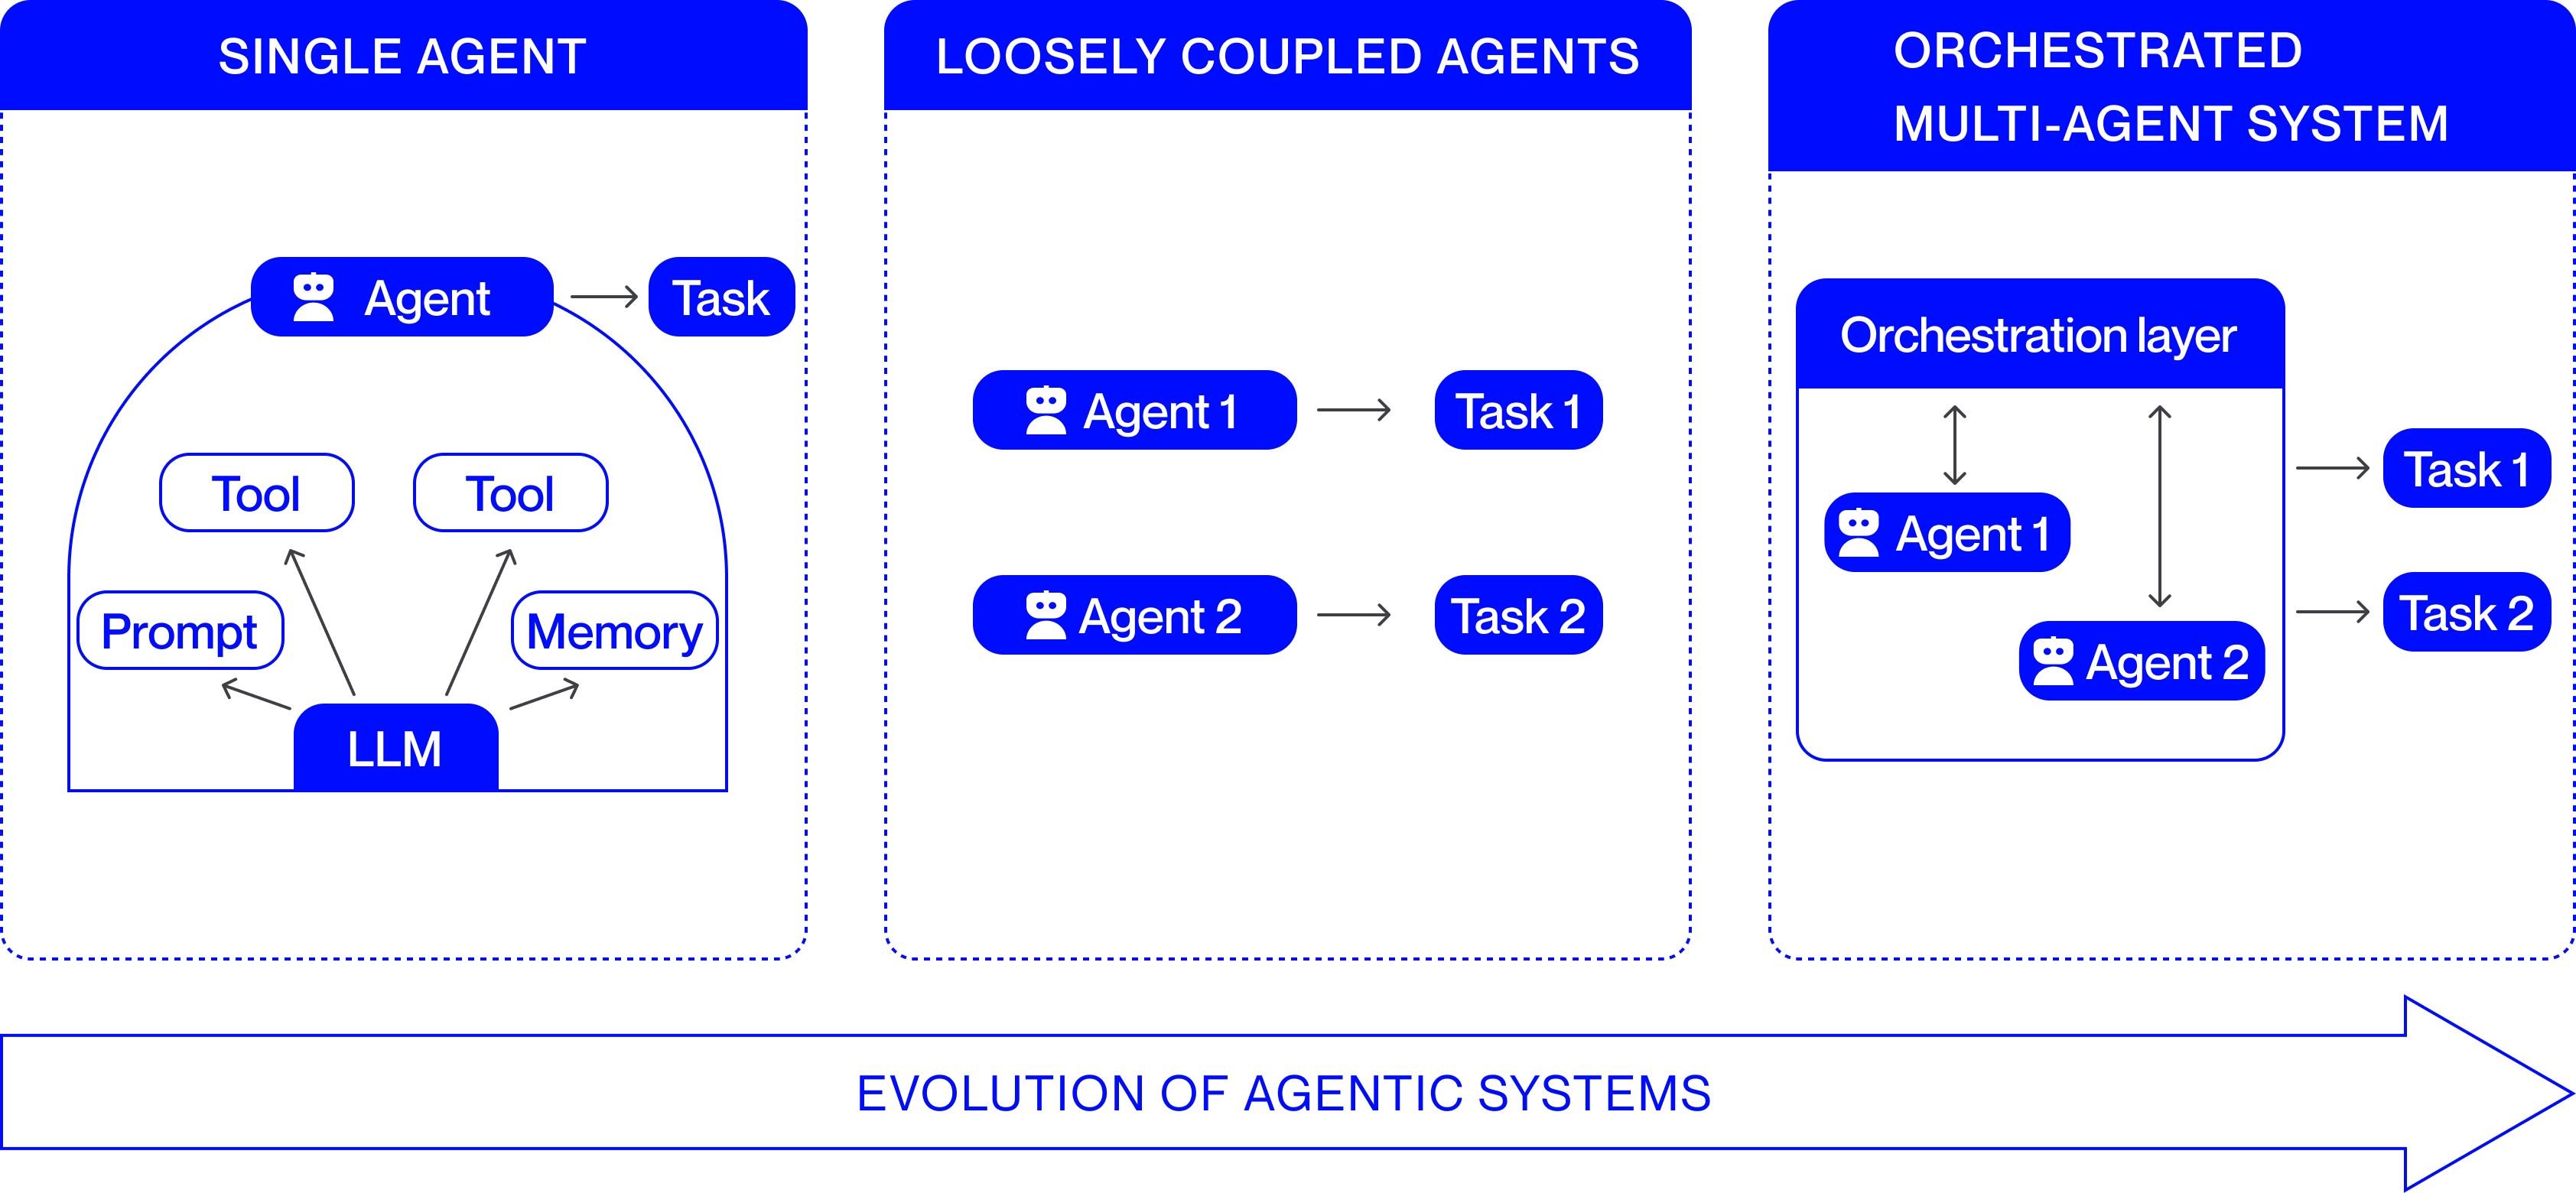
\includegraphics[width=\textwidth]{Images/chapter1/EvolutionAgenticSystems.png}
    \caption{Evolution of agentic system architectures: from a single LLM agent,
    to loosely coupled independent agents, to a fully orchestrated multi-agent system.
    Source:~\cite{agentsurvey2025}.}
    \label{fig:agent_evolution}
\end{figure}

\paragraph{Model Context Protocol.}
The \textbf{Model Context Protocol (MCP)}, introduced by Anthropic in
2024~\cite{anthropic2024mcp}, defines a standardized client-server protocol over a
\texttt{stdio} interface: tool servers expose a uniform schema describing their
capabilities, and agents discover and invoke tools dynamically at runtime. Each MCP
server encapsulates its own tools as independent, swappable modules
(Figure~\ref{fig:mcp_comparison}). In this project, MCP serves as the communication
backbone between Agent~2's ReAct loop and its web-research tool servers, enabling
search, scraping, and encyclopedic lookup through a uniform interface without any
tool-specific integration code in the agent itself.

\begin{figure}[H]
    \centering
    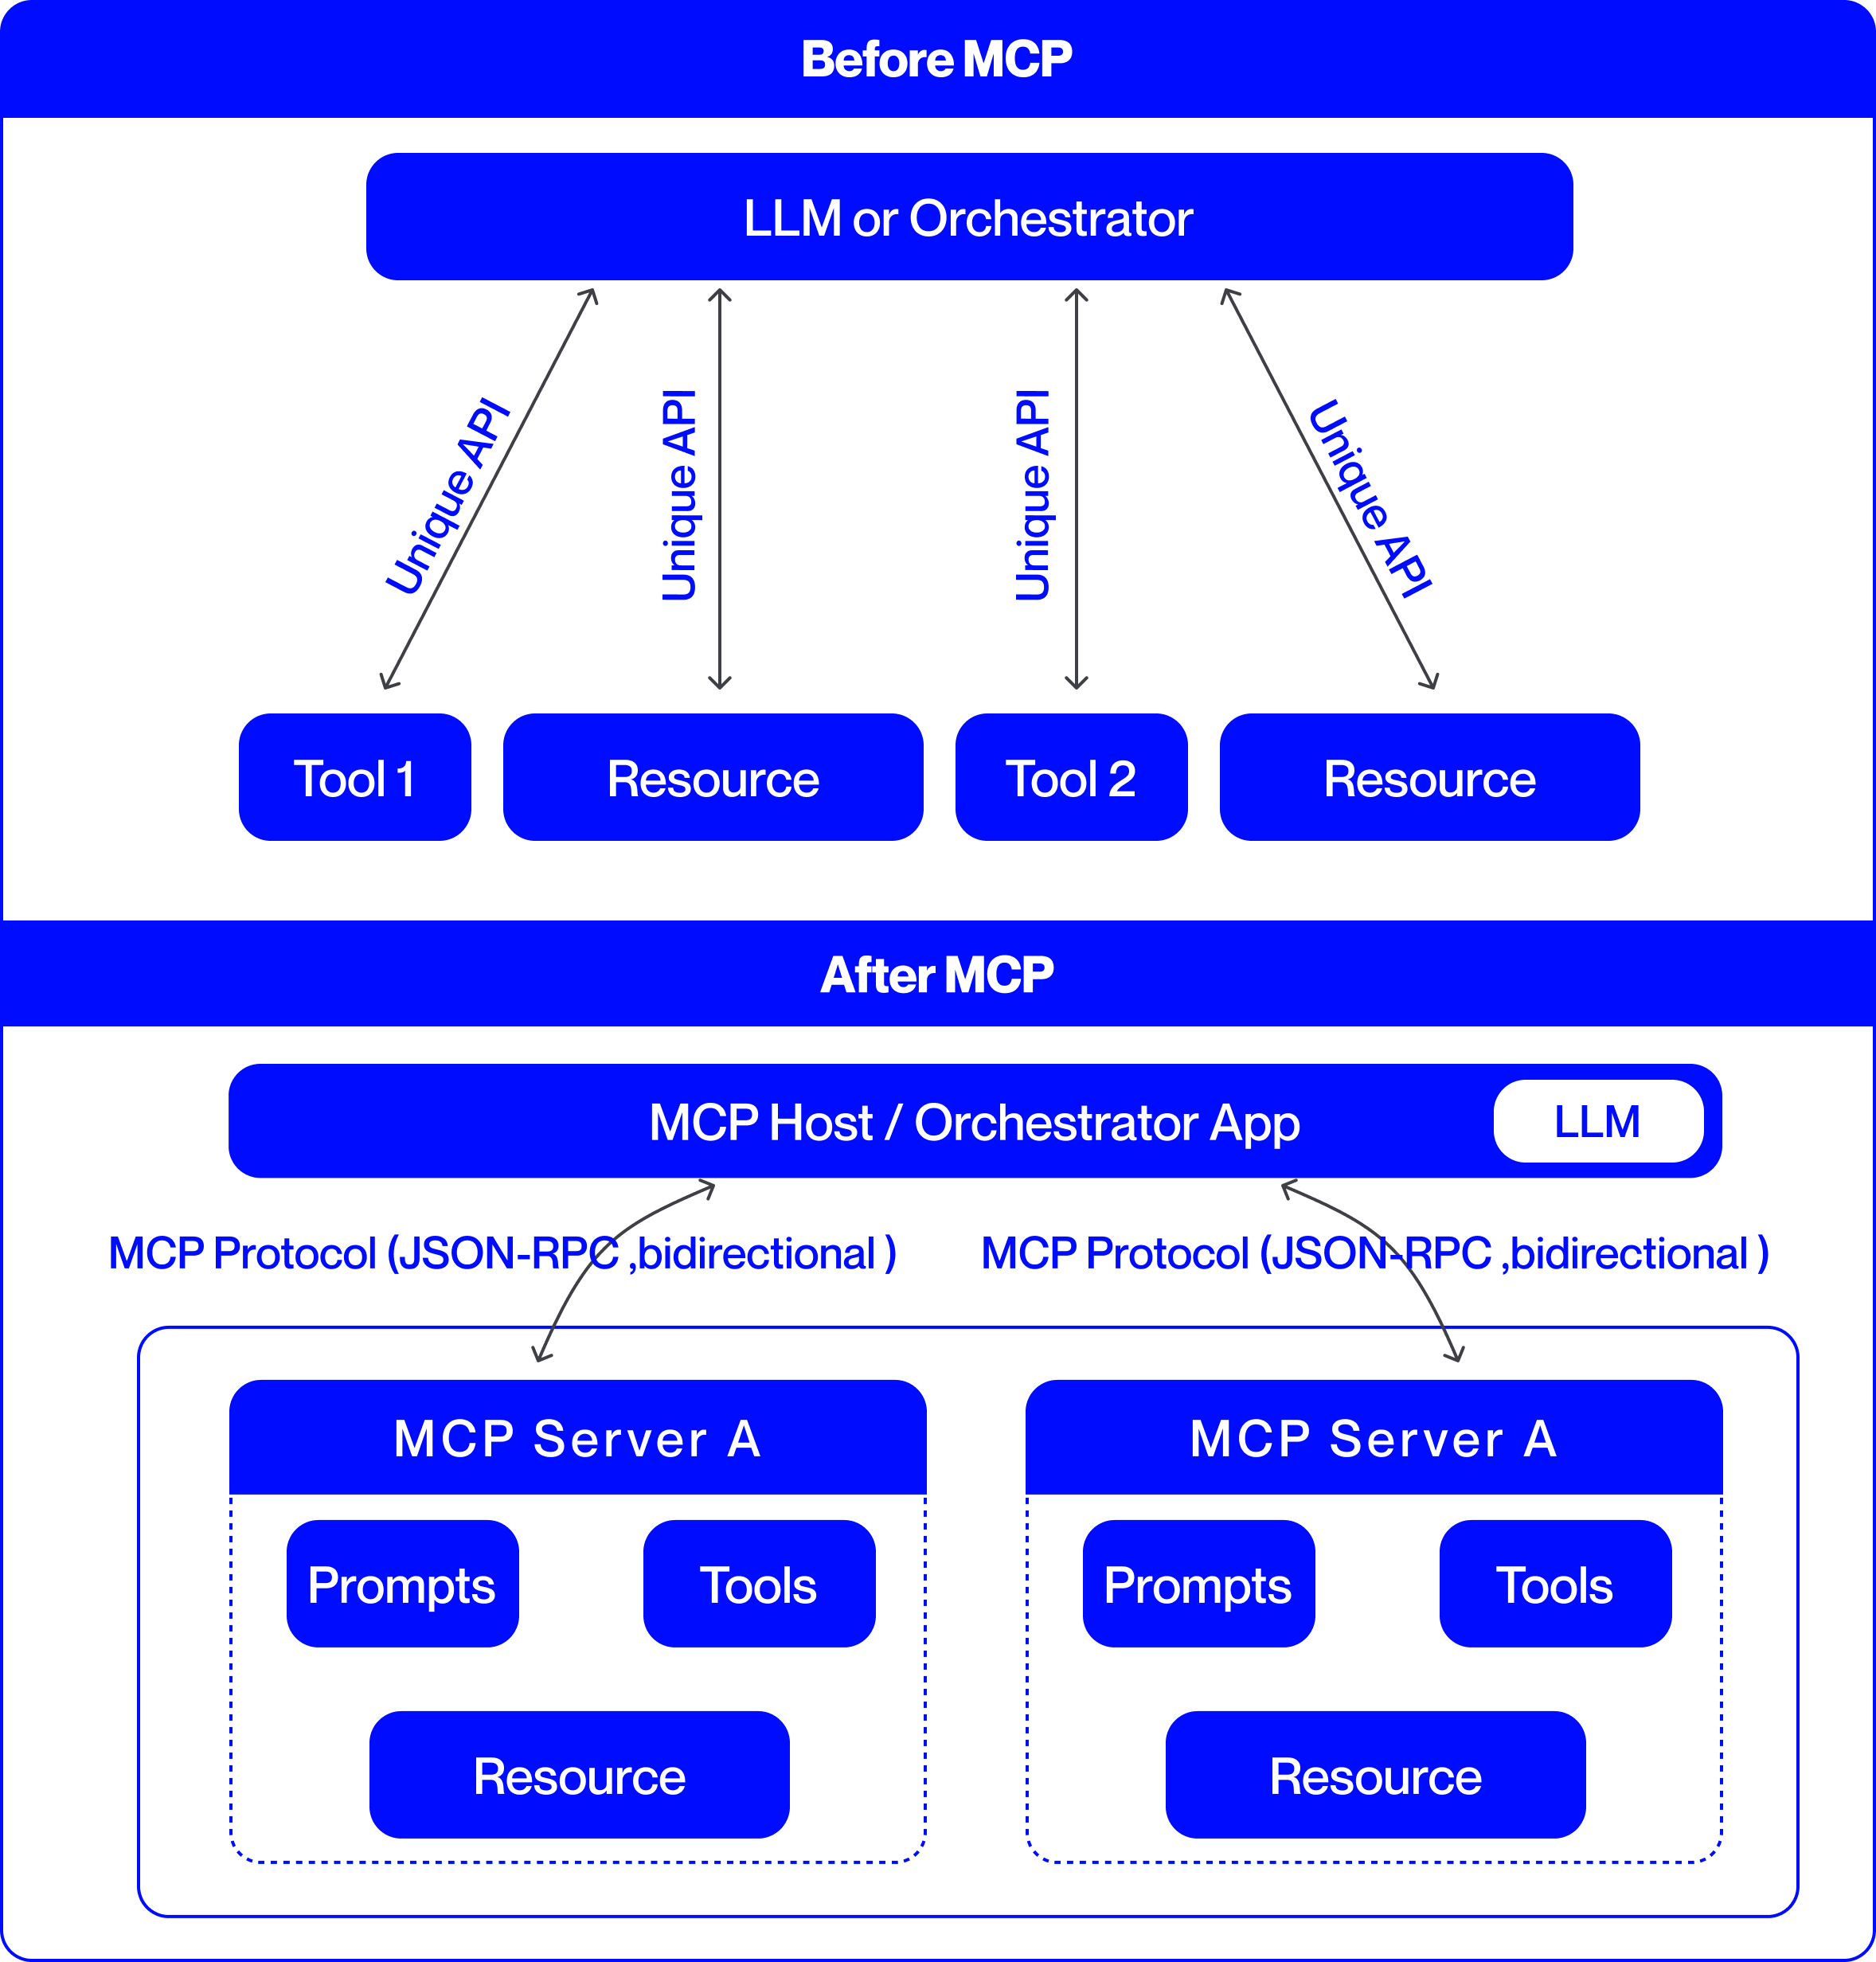
\includegraphics[width=0.7\textwidth]{Images/chapter1/BeforeVSAfter_v3.png}
    \caption{System architectures without and with MCP. Without MCP, the application
    must directly integrate each external tool. With MCP, a unified protocol layer
    mediates all interactions. Source:~\cite{agentsurvey2025}.}
    \label{fig:mcp_comparison}
\end{figure}

% ─────────────────────────────────────────────
\subsection{Related Work and Research Gaps}
\label{sec:related_work}

Despite growing interest in LLM-based visibility, no existing framework provides an
integrated, automated, and scientifically grounded solution for entity-level GEO
measurement.

\paragraph{Visual workflow automation tools.}
Platforms such as n8n~\cite{n8n2024} and Zapier support basic prompt submission and
response logging through predefined execution graphs, but offer no adaptive
decision-making, dynamic model selection, or cross-run statistical aggregation —
making them unsuitable for research-grade measurement.

\paragraph{Commercial GEO and AI visibility platforms.}
Tools including BrandGPT, Otterly.ai, and Profound monitor brand mentions in LLM
responses but with limited scientific validity: none discloses its measurement
methodology, they query a small fixed model set, and they do not support multi-run
evaluation essential for estimating mention stability~\cite{aggarwal2023geo}.

\paragraph{Summary of gaps.}
Table~\ref{tab:gaps} positions the contributions of this project against the key
limitations of existing approaches.

\begin{table}[H]
\centering
\caption{Limitations of existing approaches and contributions of the proposed system.}
\label{tab:gaps}
\begin{tabular}{|p{3.0cm}|p{4.6cm}|p{4.6cm}|}
\hline
\textbf{Aspect} & \textbf{Existing Approaches} & \textbf{This Project} \\
\hline
GEO measurement &
Manual or single-run, no cross-model analysis &
Automated, multi-prompt, multi-run, multi-model \\
\hline
Agent architecture &
Fixed execution graphs or visual workflows &
Autonomous ReAct orchestrator with runtime decision-making \\
\hline
Web data extraction &
Single source or manual lookup &
Multi-source extraction via MCP-based tool servers \\
\hline
Target domain &
Large, English-language brands &
Local entities in emerging and non-English markets \\
\hline
Statistical rigor &
Single-run, no stability analysis &
Mention rate, stability score, prominence index \\
\hline
\end{tabular}
\end{table}

Three gaps are of particular significance: no existing tool measures entity
visibility with statistical rigor across multiple prompts, runs, and models
simultaneously; no open framework automates the full pipeline from prompt generation
to web data extraction within a single autonomous system; and the relationship
between structured web presence signals and LLM visibility remains empirically
uninvestigated for local businesses in non-English markets. This project addresses
all three within a single integrated pipeline.

% ─────────────────────────────────────────────
\section*{Conclusion}
\addcontentsline{toc}{section}{\textbf{Conclusion}}

This chapter has traced the progression from link-based visibility governed by
documented algorithmic signals to representation-based visibility, where presence in
LLM-generated responses is an emergent property of training data coverage. As LLM
adoption scales globally, the asymmetry between well-represented global brands and
structurally neglected local businesses intensifies, making rigorous measurement
tools increasingly urgent. Existing approaches — visual automation platforms,
commercial monitoring dashboards, and single-model GEO tools — address this problem
only partially, each falling short in adaptability, rigor, or scope. These
limitations directly motivate the design of the system presented in the following
chapter.
